\chapter{Overview of this thesis' contributions}

\section{Methodology}

\todo[inline]{
    Study by example, human subject research, and modeling.

    Empirical research.

    Include testbeds!
}

\section{Contributions of this thesis}

\todo[inline]{
    Here's where we ``present'' the papers.
    However, we do this by presenting a ``red thread'' of contributions and key results.
    Drive towards one big picture.

    Add a hardened compilation of key results, conclusions, figures, and tables.
    Synthesize and summarize the research questions and conclusions to find the red thread.

    EdgeDroid (first demo paper at SEC, then HotMobile paper).

    Tie in CLEAVE paper here as an extension of the approach towards other latency-sensitive applications.

    Potentially include Ainur paper as a further extension of the methodology?

    PLOS ONE paper as a stepping stone towards the final goal of a more realistic model?

    Finally, EdgeDroid2 paper:
    Presents the final model of human behavior
    Applies it to a real optimization problem, employing theoretical results proved by Vishnu
}

This thesis presents seven main key contributions to the literature, which we summarize below:

\begin{enumerate}
    \item\label{item:contrib:methodology} A methodological approach to studying system responsiveness versus resource consumption trade-offs in \ac{WCA}.
    This approach is based on the emulation of the client-side workload, while maintaining the \emph{real} server-side process as well as network stack.
    \item In conjunction with the aforementioned methodology, a tool (EdgeDroid) for the emulation of human behavior in \ac{WCA}.
    This tool implements the first ever parametrizable model of human behavior for these applications using empirical data collected from a series of human-subject experiments.
    \item A characterization of the effects of individual personality differences in human responses to reduced system responsiveness in interactive systems such as \acl{WCA}.
    In particular, this thesis presents novel evidence for the modulating properties of \emph{neuroticism} on the reaction to increased delay in these systems.
    \item An preliminary, yet novel exploration of the implications of realistic modeling of human timings in \ac{WCA} applications for their optimization potential.
    \item\label{item:contrib:methodology:ncs} An extension of the methodology described in \cref{item:contrib:methodology} towards \acp{NCS}.
    \item A novel tool, CLEAVE, for the emulation of \acp{NCS} on edge infrastructure.
    This tool has been designed from the ground-up to be edge-native, implemented using widely-adopted technologies in the disciplines of cloud and edge computing.
    \item Finally, a software framework for the management and automation of the testbeds required for the methodology described in \cref{item:contrib:methodology,item:contrib:methodology:ncs}.
\end{enumerate}

\section{A methodology for the study of latency trade-offs in \acs{WCA}}

\subsection{The EdgeDroid model of human behavior}

\subsubsection{Characterizing human reaction to delays in \ac{WCA}}

\subsubsection{Implementing the model}

\subsubsection{Implications of the EdgeDroid model for \ac{WCA} optimization}

\section{A methodology for the study of latency trade-offs in \acsp{NCS}}

\subsection{The CLEAVE emulation framework}

\section{The Ainur software framework for Edge Computing testbeds}

\todo[inline]{Intro and conclusions from EdgeDroid 1.0 paper}

There is increasing interest from academia and industry in novel applications such as immersive augmented reality (AR) or wearable cognitive assistance (WCA)~\cite{Chatzopoulos:Hyperion,Ha:TowardsWearableCogAssist}, also known as human-in-the-loop applications.
These applications aim to seamlessly integrate into the lives of users to provide real-time, context-aware information by capturing user and environment information and leveraging compute-intensive algorithms to analyze the data in order to provide real-time feedback to the user.
Sensory input, such as video, audio, and other user-related data such as orientation and movement, are examples of what is typically captured, while the backend generally employs machine learning technologies such as Deep Neural Networks (DNN)~\cite{Ha:TowardsWearableCogAssist}.
\Cref{fig:pipeline2} depicts such a system.
These applications are highly latency sensitive, measuring latency as the time from the capture of the sensory information until feedback is received.
Delays above a certain threshold can hurt the user experience or even make the application unusable~\cite{Chen:AnEmpiricalStudyOfLatency}.

In literature, these challenging latency requirements have so far mainly been addressed through research on the optimal placement of the compute process.
There is a broad understanding today that with the advent of edge computing, human-in-the-loop applications will become viable~\cite{Bittmann_Edge,flinn2012cyber,Chen:AnEmpiricalStudyOfLatency,Ha:JITProvisioning}.
However, with respect to end-to-end latency, there are many more trade-offs involved than merely the question of where the compute backend is placed.
A human-in-the-loop application consists of various processing steps that can be influenced during the development of the application.
What kind of compression to apply to the sensory input on the uplink; which backend algorithms to utilize; how to stage the backend; when to send feedback to the human users; and how to manage congestion on the loop, as well as wireless channel fluctuations --- all these design choices impact the latency of the application.
There are also many design choices in the infrastructure: how is the sensory input conveyed to the point of computation (i.e.\ by which wireless system; with which transmission/prioritization scheme); which hardware is running at the backend; which operating system; how is the feedback conveyed back to the human user?
Finally, in production use these applications will most likely run concurrently with others.
How does this, together with other best-effort applications, impact the latencies perceived by the human user?
Existing studies~\cite{Ha:TowardsWearableCogAssist, Chen:EarlyImplementation, satya2009case,Chatzopoulos:Hyperion} of this class of applications have only lightly touched upon these issues~\cite{Chen:AnEmpiricalStudyOfLatency}.
On the other hand, recently published models for end-to-end latency of edge computing architectures~\cite{Zubaidy15,Schiessl17} are quite complex, while not accounting for the specifics of human-in-the-loop applications.
We only have a coarse understanding of the many degrees of freedom upon which end-to-end latency depends.

The goal of this paper is to provide a methodological approach to studying these latency trade-offs, along with a tool, EdgeDroid 1.0\footnote{We plan to make the EdgeDroid 1.0 benchmarking suite available as Free and Open Source Software and the recorded traces under a Creative Commons License.}, that simplifies the benchmarking of human-in-the-loop applications.
We view EdgeDroid 1.0 to be the very first, and simplest, of a family of tools that will embody increasingly sophisticated and accurate models of user behavior.

Due to the complex nature of the applications and the infrastructure, we opt for experimentally studying the trade-offs in a repeatable and controllable fashion.
This is difficult mainly due to the unpredictable reaction of human users to the feedback from the backend --- a user might very well misinterpret the feedback handed to them.
EdgeDroid 1.0 mimics the operation of human-in-the-loop applications by replaying recorded traces of sensory input.
This sensory information is then processed by the original compute process at the backend, generating feedback.
However, this feedback is not processed by humans, but by a parameterizable model of human reaction.
Through synchronized time tracking at the different processing points of the application, EdgeDroid 1.0 allows for accurate measurements of key performance metrics such as the distribution of delays across the application pipeline.
Analysis of these metrics can be performed down to the individual input sample, allowing us to zoom into the internal model of the application under consideration.
Thus, EdgeDroid 1.0 allows us to illuminate the many latency trade-offs existing at the level of the infrastructure, as well as the level of the application.
It can also be used for debugging and validation, by comparing the expected execution flow of a particular trace with the actual flow during the benchmarking.
To the best of our knowledge, this experimentally-driven benchmarking approach is the first one towards experimental performance characterization and potential optimization of human-in-the-loop applications

Benchmarking human-in-the-loop applications is hard, given their tight interaction with human users who complicate the scaling and repeatability of experiments.
In this paper, we have presented a benchmarking suite for this type of applications, called EdgeDroid 1.0, capable of cutting out the need for users in performance evaluations.
We achieve this by employing pre-recorded sensory input traces which we play over the network to the real application backend, employing a parameterized user model to react to feedback.
We demonstrate its utility through a series of use case scenarios, from which we are able to extract metrics regarding latency both in regards to the application itself and the hardware stack.
We believe the EdgeDroid 1.0 suite thus represents an important first step towards enabling inexpensive and low-complexity large-scale research on the scaling limits of this type of applications, a requirement for wide adoption of the technology.

Nonetheless, there is still future work to be done.

The user model presented in this paper is only preliminary, and we are currently conducting research in characterizing user behavior when interacting with WCA applications in order to present a more complete model in the future.
As mentioned in \Cref{sec:implementation}, in EdgeDroid 1.0, our model is that of a user who does not suffer any of the shortcomings of real human users such as annoyance, fatigue, frustration, nausea.
Rather, EdgeDroid 1.0 models a perfectly stoic user who is like an automaton and responds in a precisely reproducible and deterministic manner to the same system stimulus every time.
Of course, no real human user is an automaton.
In the future, we envision creating  many versions of EdgeDroid (i.e., EdgeDroid 2.0, EdgeDroid 3.0, etc.) that embody more human-like user models that more accurately emulate attributes such as those mentioned above.
Experimental validation of these human-like user models via user studies will be an important part of our future work.

We are also working on expanding the benchmarking suite to also work first with other types of Wearable Cognitive Assistance, and later with other categories of human-in-the-loop applications.
Other types of WCA we will consider in future iterations of the tool include real-time task-assistance WCA applications (such as the Ping-Pong application described in~\cite{Chen:EarlyImplementation}), which don't have a linear task model like task-guidance WCA and have tighter latency bounds and context- and information-providing WCA applications, for instance, applications which recognize faces and provide relevant social-media information related to that person.
The latter also do not have a linear task model, but present more lax latency bounds.

\todo[inline]{Intro and conclusions from CLEAVE paper}

\begin{figure*}
    \centering
    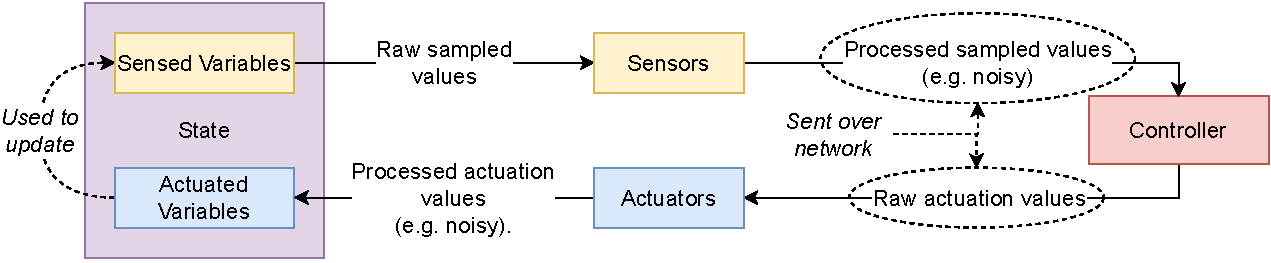
\includegraphics[width=.8\textwidth]{publications/2022CLEAVE/images/CLEAVE_NCS_structure}
    \caption{
        Structure of an emulated \acl*{NCS} in \acs*{CLEAVE}.
    }\label{fig:cleave:ncs:struct}
\end{figure*}

The number and applications of \acp{CPS}~\cite{Rajkumar2010CPS} --- i.e.\ systems in which a real, physical mechanism is controlled by a computer --- have exploded in recent years.
However, this rapid increase in adoption has mostly been limited to industrial contexts.
Although \acp{CPS} present huge opportunities for all facets of society, they have yet to reach our daily lives in any relevant scale due to their stringent operational requirements.
This is about to change, however, as with the advent of novel wireless communication technologies as well as networking paradigms, such as cellular 5G and edge computing~\cite{Satya2017Emergence}, consumer-grade \acp{CPS} will be made possible.
These technologies meet two key requirements of \acp{CPS}: real-time capabilities (through extremely low end-to-end latencies), and context- and locality-awareness, and will most likely become the backbone of \ac{CPS} in the future.

\acp{NCS}~\cite{Gupta2010NCSOverview}, a type of \ac{CPS} wherein multiple networked actuators and sensors form a part of the same automatic control system will benefit from the adoption of these technologies.
Depending on the physical system being controlled, \acp{NCS} can have stringent timing and reliability requirements for communication that conventional cloud paradigms and cellular networks cannot meet~\cite{Wan2020Efficient}.
This necessitates sophisticated tools for the performance evaluation of future system architectures, as well as novel NCS design paradigm.

%Due to their potential advantages for industrial and commercial settings, there exist works~\cite{Zhang2016Survey} dedicated to the modelling and performance characterization of \acp{NCS}, improving NCSs by distributing control functions across networks, facilitating centralized coordination, control, and monitoring.

One the one hand, related literature in \acp{NCS} leverages to a large extent theoretical models, at the price of being able to capture networked systems effects only on a coarse level. 
%follows a theoretical approach, and only a small fraction of it deals with experimental studies.
On the other, there exist several approaches when considering experimental methodologies. 
%A number of works concerning \acp{NCS} deal with experimental studies.
%\acp{NCS} have an inherently inter-domain nature intertwining knowledge from the fields of communications, computing, and control theory in ways that cannot be studied in isolation, leading to various different approaches to such studies.
One such approach uses setups in which the complete system is built on top of real hardware.
This approach is employed in the works of Baumann \emph{et al.}~\cite{Baumann2018LowPower} and Cuenca \emph{et al.}~\cite{Cuenca2019UAV}; in both of these, the authors implement their approach on physical testbeds.
Conversely, other studies choose to instead use completely \emph{simulated} \ac{NCS} setups.
The authors in\ \cite{Ma2019DynamicSched} have opted for such an approach.
These studies often employ combinations of physical and network simulation tools trying to capture the complex dynamics of \acp{NCS}.
Finally, some experimental studies instead employ \emph{virtualized} approaches, in which either
\begin{enumerate*}[itemjoin={{; }}, itemjoin*={{; or }}]
    \item a real network interacts with a simulated or emulated control system~\cite{Wang2020VoltageControl}
    \item a simulated network interacts with a real control system~\cite{Natale2004InvPendEthernet}.
\end{enumerate*}

As evidenced above, experimental research in \acp{NCS} includes varied heterogeneous hardware and software platforms, methodologies and key performance indicators.
This, in turn, leads to hardware, software, and methodology fragmentation, as different studies tend to prefer approaches more favored in their respective communities.
Furthermore, existing studies tend to focus on individual aspects and components of a system, thus producing results which do not provide a complete image of the \ac{NCS}.
This has caused a gap in knowledge pertaining to the reproducibility and comparison of experimental studies on these systems.

Zoppi \emph{et al.}~\cite{Zoppi2020NCSBench} made the first (and to the best of our knowledge, the only) attempt at tackling this challenge in their work.
In their work, they proposed a platform called NCSBench, to be used for reproducible benchmarking in NCS.\ 
Their methodology utilizes joint knowledge of control, computation, and communication. 
In their work various architectural elements and the corresponding delays associated with the NCS are modelled. 
Multiple experimental parameters and certain observable key performance indicators are defined and utilized in the implementation. 
This work however utilizes a physical LEGO\textregistered{}\ Mindstorms EV3 Core Set\texttrademark{}\  based plant for the implementation, preventing instantaneous changes in plant characteristics and component parametrizations.
Furthermore, relying on physical objects like an inverted pendulum limits scalability of the experimentation in practice. 

We overcome this issue by proposing a completely virtual plant allowing for unparalleled flexibility in changing the plant model and characteristic features of the experiments.
In this paper, we present the first fully-software-based framework for scalable and repeatable benchmarking of edge-native \ac{NCS}.
As edge computing begins being adopted by industry, more and more variations have begun to appear in literature.
``Near'', ``far'', ``core'', and ``telco'' edge describe variations of the original concept and are becoming ubiquitous in new research.
While the core idea of edge computing is widely accepted as fundamental for pervasive \acp{NCS} in general, understanding the strengths and weaknesses of such different edge concepts is of paramount importance.

Our framework, \ac{CLEAVE}, aims to simplify the repeatable and scalable benchmarking of such systems.
It is fully virtualized, inspired by our previous work on benchmarking human-in-the-loop applications on the edge~\cite{Olguin2019EdgeDroid}.
The tool consists of a benchmarking framework and software development kit for the development of emulated physical systems and softwarized controllers.
These virtual \acp{NCS} can then be deployed on real networks for reparametrizable, repeatable, and reproducible benchmarking of the complete system.

\ac{CLEAVE} is built using \emph{Python 3.8}, making it highly extensible and able to harness the multitude of already existing user libraries.
It is furthermore compatible with container technologies such as \emph{Docker}\footnote{Docker Engine: \url{https://www.docker.com/}}, making it suitable for automated deployment, scaling, and benchmarking on industry-standard edge setups using container orchestration solutions.

The rest of this paper is structured as follows.
\cref{sec:approach} presents the design principles and implementation of the framework.
In \cref{sec:experiments}, we present a use case scenario which validates the utility, flexibility, and repeatability of \ac{CLEAVE}.
Finally, in \cref{sec:conclusion} we conclude this work.

The issue of repeatable and scalable benchmarks has been largely glossed over in \ac{NCS} literature, as existing experimental research studies tend to implement \emph{ad-hoc} solutions.

In this work, we aimed to tackle this issue through a fully software-based framework for repeatable, reproducible, and easily scalable \ac{NCS} benchmarking with a particular focus on edge deployment.
We argue our approach, \ac{CLEAVE}, embodies a better solution than previous work for a number of reasons:
\begin{enumerate}
    \item Compared to fully physical approaches, such as those used in\ \cite{Baumann2018LowPower} and\ \cite{Cuenca2019UAV}, our approach allows for greater flexibility and scalability.
    The aforementioned approaches rely on specialized and sometimes entirely custom-built physical platforms, and although flexible and cheap approaches such as Zoppi \emph{et al.'s} --- which uses a LEGO-based physical plant --- exist, these still do not reach the level of flexibility afforded by a fully software-based framework. 
    Experimenters still need copies of the hardware, making anything other than small-scale setups unfeasible.
    In contrast, our approach requires only general-purpose computing platforms, and can be employed by basically anyone with access to a computer.
    Scalable deployments can in turn easily and cheaply be set up using single-board computers and/or virtual cloud instances.
    \item When compared to simulated approaches such as\ \cite{Ma2019DynamicSched}, \ac{CLEAVE} provides a higher level of realism, in particular with regards to the network segment of the system.
    \item Finally, although it shares much in common with previous emulated approaches such as the one employed in\ \cite{Wang2020VoltageControl}, \ac{CLEAVE} has an advantage by specifically targeting a general-purpose approach using industry-standard, cloud- and edge-native tools and software.
    The tool can easily be deployed and scaled using widely-used frameworks such as Docker Swarm and Kubernetes.
\end{enumerate}

We validate the utility of this tool through an example use case approximating a proposed edge deployment of inverted pendula control loops co-located with video analytics services.
We argue such a use case represents a realistic scenario and appropriate benchmark for the tool, since
\begin{enumerate*}[itemjoin={{; }}, itemjoin*={{; and }}]
    \item the inverted pendulum plant is ubiquitous in \ac{NCS} research
    \item similar setups exist in real-world industrial use
    \item video analytics has long been proposed as a ``killer app'' for edge computing.
\end{enumerate*}
Our results showcase the ability of the framework to extract relevant metrics relating to the stability of the control system, as well as on the performance of the underlying network link.
We believe \ac{CLEAVE} represents an important step towards enabling inexpensive and low-complexity scalable research for real-world deployment of edge-bound \acp{NCS}.

There is still, however, work to be done.
We are extending the number of plant and controller implementations on the framework, with the goal of creating an open library of \acp{NCS} to share with the community.
At the moment, the interactions of \ac{CLEAVE} and tools such as Docker are still quite superficial.
Our goal is to achieve a much tighter integration, e.g.\ by providing the toolkit as pre-packaged container images.
Finally, the validity of the results obtained by the framework will have to be verified through more thorough, realistic scenarios than what we have been able to show in this work.
In particular, we intend to perform large-scale experimentation targetting 5G cellular deployments, as this technology is set to become the backbone of edge networks in the near future.

\todo[inline]{Intro and conclusions from Ainur paper}

Experimental research in the area of wireless networking has received ever increasing attention over the last years, driven, on the one hand, by the complexity of modern networked systems and corresponding applications. 
On the other, networked systems are more and more based on software instead of dedicated hardware, which allows experimental testbeds to be rededicated simply through an update as system versions evolve --- in contrast to the redeployment of hardware necessitated \numrange[range-phrase={--}]{10}{15} years ago.
The complexity of these systems, as well as their softwarization are expected to continue growing, driving in turn an expanding interest in testbed-based experimental research in wireless systems.

Over the last years, several small- to mid-scale testbeds have emerged that leverage a large degree of freedom with respect to hardware and software, for example, the 
\begin{enumerate*}[itemjoin={{, }}, itemjoin*={{, and }}]
    \item \acs*{COSMOS}
    \item \acs*{POWDER}
    \item \acs*{ARA}
    \item Drexel Grid \ac{SDR}
\end{enumerate*} testbeds.
\acs{COSMOS}~(\emph{\acl{COSMOS}})\acused{COSMOS} is a testbed spanning an area of roughly \num{1} square mile (\SI{2.6}{\kilo\meter\squared}) featuring \acp{SDR}, \si{\milli\meter}-wave equipment, optical fibers, cloud integration, and compute for core network functionality and application data processing~\cite{Cosmos1,cosmos2}.
It contains over \num{200} rooftop, intermediate, and mobile nodes, and is controlled and managed by a central node.
\ac{COSMOS} relies on the \ac{OMF} (originally developed for ORBIT~\cite{orbit}), and employs the \ac{OEDL}, a domain-specific imperative language based on Ruby, for experiment development and definition.

\acs{POWDER}~(\emph{\acl{POWDER}})\acused{POWDER} promises research on wireless and mobile networks with a level of programmability down to the waveform~\cite{powder}.
The testbed spans a \SI{15}{\kilo\meter\squared} area and features about \num{15} fixed programmable radio nodes, based on off-the-shelves \acp{SDR} and featuring edge-like compute capabilities and integration with cloud resources, which interact with \num{50} mobile nodes. 
\ac{POWDER} experiments are defined and developed in \emph{profiles}, which correspond to \ac{VM} images containing the necessary software and configurations.
These profiles are defined through using \ac{RSpec}\footnote{\url{https://groups.geni.net/geni/wiki/GENIExperimenter/RSpecs}} documents.

The \ac{ARA} platform is an at-scale testbed for wireless research spanning a rural area with a diameter of over \SI{60}{\kilo\meter} in Iowa~\cite{zhang2022ara}.
Its core goal is the study and deployment of advanced wireless platforms and technologies in real-world agricultural and rural settings.
It includes a broad range of wireless platforms ranging from low-\ac{UHF} massive \ac{MIMO} to \unit{\milli\meter}Wave, deployed through both \acp{SDR} and programmable \ac{COTS} radios, as well as automated ground vehicles, cameras and sensors.
\ac{ARA}'s software stack, ARASoft, is based upon the highly flexible and powerful \ac{CHI} software suite from the Chameleon testbed project~\cite{keahey2020lessons}, which in turn is based on the widely adopted OpenStack~\cite{openstack} cloud-computing framework.
This affords the \ac{ARA} testbed a high degree of flexibility, as well as lowers the learning curve for new contributors and users.

Finally, the \emph{Drexel Grid \ac{SDR} Testbed} features \acp{SDR} that connect either over-the-air, through a channel emulator, or over a combination of the two, to facilitate realistic and reproducible experimentation~\cite{DrexelGrid}.
Primarily intended for \ac{SDR}-centric research, it does not integrate any core, cloud or edge components.
However, the testbed extensively employs the \ac{LXC} runtime for the deployment of both experimental code and \ac{SDR} software, which affords users great freedom when it comes to the development of experiments.

Experimentation is key to to fully understanding the implications of next-generation wireless systems, cloud, and edge computing paradigms, and thus more of these testbeds are sure to emerge in the near future.
Yet, little work has so far been devoted to general-purpose, hardware-agnostic software frameworks for the management and automation of such systems.
Existing platforms implement their own, ad-hoc software solutions which are not compatible with other testbeds, and in many cases are not even compatible with reigning cloud-native standards.
This is, for instance, the case with \ac{COSMOS} and \ac{POWDER}; their reliance on domain-specific languages limits their integration with cloud-native solutions, which generally build upon general-purpose languages such as Python and Go.
These testbeds further leverage virtualization technology based on \acp{VM} instead of more lightweight and edge-compatible solutions such as containers.

To the best of our knowledge, CloudRAFT~\cite{cloudraft} is the only work to tackle (to a certain extent) this challenge.
CloudRAFT corresponds to a cloud-based framework for mobile network experimentation, with a focus on simplifying the management of testbed resources.
The goal of this project is to integrate, coordinate, share, and improve upon existing testbeds; and employs pre-built \acp{VM} containing the necessary software for experiments.
Although it provides some automation for testbed resource provisioning and experiment execution, its focus is largely rather on the sharing and partitioning of testbed systems.
Testbeds currently working with CloudRAFT include a variety of domain-specific setups, including \iac{SDR}-based testbed as a well as a ground vehicular robot for mobility-related experimentation.

In this work, we present our solution to the challenge of testbed automation: Ainur, a framework for wireless testbed automation with a specific focus on end-to-end experimental research in the context of edge-computing using cloud- and edge-native technologies.
Ainur is designed to deploy experimental runs from a workload perspective by configuring the physical testbed, initializing all involved software components, deploying and executing the experimental workload, collecting logs and data, and finally gracefully degrading the system.
The framework allows for dynamic, software-definition of physical and logical links, network topology, cloud and edge computing resources, as well as experimental workload deployment and orchestration.
It heavily leverages cloud-native technologies, such as Docker containers, in order to support a wide variety of different testbed hardware setups and experimental configurations and workloads, as well as to be as easily extendable as possible.
Furthermore, we make Ainur available to the community as \ac{FOSS}.
It can be obtained from the {KTH-EXPECA/Ainur} repository on GitHub~\cite{ainur:github}, released under an Apache version \num{2.0} license.

The rest of this paper is structured as follows.
\cref{sec:ainur} presents the framework as well as the key concepts and technologies supporting its design and architecture.
This section also discusses briefly the assumptions made about the underlying hardware on which the framework is set to run, and we present an overview of our experimental testbed.
Next, \cref{sec:demo} describes two demonstration procedures through which we will showcase the flexibility and potential of this tool for the automatic, repeatable, end-to-end experimentation in the context of wireless testbeds.
Finally, in \cref{sec:conclusion} we summarize our contributions, discuss future directions, and conclude this paper.

In this paper, we have introduced a framework for repeatable end-to-end testbed automation in the context of wireless networking and edge computing research.
Named Ainur, it simplifies the execution and verification of end-to-end experimentation by automating the
\begin{enumerate*}[itemjoin={{; }}, itemjoin*={{; and }}]
    \item establishment of physical links between hosts, including the configuration of complex wireless systems such as 4G \ac{LTE} and 5G
    \item provisioning of and connection to remote cloud instances
    \item initialization of \ac{IP} layer connectivity between hosts
    \item collection of logs and data
    \item deployment, scaling, and lifecycle management of containerized processes
\end{enumerate*}.
We have described its general architecture, which follows a layered design mimicking the network stack layers the framework directly interacts with, as well as the underlying assumptions about its deployment environment and specific requirements for its deployment.
We have also outlined a demonstration which showcases the flexibility and power of the framework by deploying two different workloads to our testbed.
We believe our framework represents an important step towards repeatable, replicable, yet low-access barrier end-to-end wireless testbed experimentation.
It has been released as \ac{FOSS} and can be found on GitHub~\cite{ainur:github}.\\

In terms of future work, our current efforts are focused on the expansion and integration of Ainur with \ac{CHI}~\cite{keahey2020lessons}.
While we believe Ainur to be unique and valuable in its focus on fully-automated end-to-end wireless edge computing experimentation, integrating with the above software stacks will provide a number of features and functionalities which will greatly expand Ainur's potential.
Features like resource reservation, multi-tenant testbed access, and automated bare-metal and \ac{VM}-host instantiation will make Ainur better suited for larger scale experimentation and allow us to expand the research domain targeted by the framework.
Our ultimate goal is to eventually provide Ainur as a service running inside an OpenStack/\ac{CHI} environment, leveraging the flexibility of the platform to automate the reservation of resources, instantiation of nodes and networks, execution of experiments, and final collection of results.

\todo[inline]{Intro and conclusions from PLOS paper}

Wearable Cognitive Assistants, WCA for short, have recently started to garner attention from the research community~\cite{Ha:TowardsWearableCogAssist,Chen:EarlyImplementation}.
They represent a novel category of highly interactive and context-sensitive augmented reality applications, that aim to amplify human cognition in both day-to-day tasks and professional settings.
Their mode of operation is analogous to how GPS navigation systems guide drivers, by seamlessly providing relevant instructions and feedback relating to the current task at hand.
Note that this implies seamless interaction with the context of the user --- at no moment does the user need to trigger an update explicitly, as the application is constantly tracking the state of the target task.
An example is an IKEA Assistant~\cite{IKEAAssistant} which monitors the assembly of a piece of furniture in real time, providing timely, step-by-step feedback to guide the user toward completion.

WCA systems were originally inspired by assistive use cases for people suffering from some form of cognitive decline, either through aging or because of traumatic brain injuries~\cite{Ha:TowardsWearableCogAssist,satya2019augmenting}.
More recently, they have been applied to a broader range of use cases, including step-by-step guidance on complex assembly tasks~\cite{Chen:AnEmpiricalStudyOfLatency}.
Non-wearable augmented reality and cognitive assistance systems have already been proven to be valuable tools in the industrial workplace~\cite{funk2015caworkplace,gorecky2011cognito}.
Detethering this assistance from its current fixed location will surely make it available to many more fields. 

Based on these use cases, we identify three main requirements for WCA:\@
\begin{enumerate}
    \item\label{item:pervasive} WCA systems should be available whenever the user requires them, without being tethered to a particular physical location. Assistants need to be pervasive and mobile.

    \item\label{item:interaction} Interaction with the system should be immersive and seamless, i.e.\ the assistant should be able to analyze the current context and automatically provide relevant feedback without explicit commands from the user.
    In this sense, WCA is expected to operate much like a human assistant would, by observing the performance of the user and offering guidance proactively.

    \item\label{item:lowlatency} Feedback should be ``quick'', relative to the task at hand. 
    This requirement is further strengthened by the previously mentioned ``seamless interaction'' characteristic of these systems.
    This means that users will have expectations of constant, immediate feedback as they progress through the task.
    In the case of a step-by-step task like IKEA, delayed feedback might simply confuse or distract the user.
    However, in a highly interactive task like a \emph{Ping-Pong assistant}~\cite{PingPongAssistant, Chen:EarlyImplementation} late guidance is at best a nuisance and at worst a severe handicap.
\end{enumerate}

\cref{item:pervasive} implies use of lightweight and low-power devices, preferably a wearable device that frees both hands for work.
\cref{item:interaction}, on the other hand, suggests a level of context sensitivity and proactivity that can only be provided by real-time analysis of sensor inputs such as video and audio feeds.
The compute-intensive processing suggested by \cref{item:interaction} cannot be met by the lightweight wearable devices suggested by \cref{item:pervasive}.
Only by offloading computation from a wearable device to cloud-based or edge-based infrastructure can this circle be squared.
However, offloading implies an extended end-to-end pipeline with many potential sources of queueing, transmission, and processing delays.
\cref{item:lowlatency} therefore emerges as a key concern, requiring deep understanding of the impact of end-to-end delays on WCA users.

% However, additional challenges remain in the path toward widespread adoption.
\cref{item:lowlatency} forms the base motivation for the research presented in this paper.
We still have a very limited understanding of how humans react to delays in these systems --- specifically, how changes in system responsiveness impact users.
\emph{System responsiveness} here denotes a qualitative scale ranging from \emph{high} (that is, not subject to delay or subject to negligible delay with respect to human perception) to \emph{low} (i.e.\ subject to considerable delay).
% Conversely, QoE is understood to range from \emph{good} (i.e.\ users enjoy interacting with the application) to bad (users dislike interacting with the application).
Characterizing the relationships between system responsiveness and user behavior and quality of experience is of paramount importance for the design and evaluation of these applications.
It is generally acknowledged, for instance, that a system going from a state of high responsiveness to one of low responsiveness can cause a drop in quality of experience~\cite{dabrowsky:2011:40years}. 
Furthermore, this could cause users to modify the temporal paramaters of their behavior when interacting with the system, generating a sort of \emph{feedback loop} between user and system.
A clear understanding of these relationships would allow, for instance, for the development of strategies for load balancing and optimization for large-scale deployment of WCA.\@
% Although maximizing QoE through over-engineered systems and networks would be a ``simple'' solution to this problem, in practice, the prohibitive costs of infrastructure make finding the optimal trade-off between QoE and cost a valuable endeavor.

This paper builds upon preliminary work in the field of time perception and delay characterization of WCA.\@
We expand upon the findings of Ha et al.~\cite{Ha:TowardsWearableCogAssist}, who identified the need for low-latency offloading in WCA, and of Chen et al.~\cite{Chen:AnEmpiricalStudyOfLatency}, who outlined the bounds for ``noticeable'' and ``unbearable'' latencies in these systems.
While these bounds present a general understanding of when it is likely that a user will stop using an application, they do not provide any insights as to what happens \emph{before} that --- i.e.\ how human behavior changes with system responsiveness.
We aim to tackle this gap in knowledge through the characterization of human responses to delays in the application pipeline, using latencies in the range defined by the previously established bounds.
This is an important step toward a more systematic understanding of human behavior in this domain.

We present in this paper the design and elaboration of an experimental WCA test-bed.
This test-bed was subsequently employed in a study in which undergraduate students of diverse fields of study, aged between 18 and 25 years old, were asked to interact with and follow the instructions given to them by a cognitive assistant.
Unbeknownst to the participants, we altered the responsiveness of the system in real-time and recorded the resulting behavioral and physiological reactions. 
The participants wore an array of biometric sensors measuring physiological responses that have proven useful in assessing cognitive workload during human-computer interaction~\cite{haapalainen2010psycho,kumar2016measurement} such as heart rate and EEG.\@

Through this experimental set-up, we intended to answer four core research questions relating to human responses to decreased application responsiveness.

\begin{itemize}
  \item \emph{Do subjects change the temporal profile of their actions in relation to system latency?}

  In line with previous research in this area, we expected subjects to change their temporal profiles as system responsiveness decreased.
  The extent or form of these changes were however unknown.
  We also hypothesized that large enough drops in responsiveness could lead to complete abandonment of the task by subjects.

  Our results show an emergent pacing effect on user actions as system responsiveness is reduced.
  While it would seem self-evident that users take longer to complete a task while using a system with low responsiveness --- as they have to wait longer for new instructions --- our study found that user slow-down represents a source of substantial additional delay.
  To be more precise, the data indicate that users slow down not only because they have to wait for the system to catch up, but that their reactions to new instructions is also delayed.
  Moreover, this effect scales with the decrease in responsiveness and remains for a while, even after system responsiveness improves.
  
  \item \emph{Do subjects show signals of arousal in physiological responses to changes in system latency?}
  
  We hypothesized subjects would show signs of stress and frustration as system latency increased, due to the added annoyance of dealing with an unresponsive system.

  The results we present, however, seem to refute this hypothesis. 
  We were not able to detect any significant effects on the physiological signals obtained from the biometric sensors as sytem responsiveness was altered.
  
  \item \emph{Are responses to delay effects in subjects mediated by cognition and/or emotion?}
  
  In line with previous items, we expected delay effects in subjects to be mediated primarily by emotion.
  In particular, we expected emotional effects to be correlated with the strength of the added delay.

  The results point in a different direction though, indicating that reduced responsiveness in WCA systems leads to a disruption of participants' cognitive plan for the task and not to an emotional response.
  This is evidenced by the previously discussed pacing effect and the lack of significant physiological responses.

  \item \emph{Are these effects mediated by personality indicators in any way?}
  
  Finally, we hypothesized that the individual trait of \emph{neuroticism}~\cite{john1999:bfi} would play a role in mediating these effects, as it has previously been connected to intolerance for time delay~\cite{hirsh2008delay}.
  We also expected \emph{focus} and \emph{involvement}~\cite{witmer1998:itq} to play roles in this.

  The results obtained agree with our hypothesis. 
  We found significant effects of neuroticism on the responses exhibited by subjects, and all three traits were found to play a role through factor analysis.

\end{itemize}

% Our results indicate that reduced responsiveness in WCA systems leads to a disruption of participants' cognitive plan for the task.
% This is evidenced by an emergent pacing effect on user actions as system responsiveness is reduced.
% While it would seem self-evident that users take longer to complete a task while using a system with low responsiveness --- as they have to wait longer for new instructions --- our study found that user slow-down represents a source of substantial additional delay.
% To be more precise, the data indicate that users slow down not only because they have to wait for the system to catch up, but that their reactions to new instructions is also delayed.
% Furthermore, this effect persists for a while after system response improves and is modulated by intrinsic personality traits, in particular, \emph{neuroticism}~\cite{john1999:bfi}. 

We believe that these results provide concrete and relevant implications for WCA design, deployment, and optimization.
One example is the behavioral slow-down, as it extends application runtime significantly, and thus has clear and direct implications for resource and power consumption.
Another is the fact that the adverse effects of delay on users do not immediately subside as delay is diminished --- this has potential consequences for resource allocation strategies.
Moreover, in multi-user scenarios, the dependency of user slow-down effects on delay mean efficient resource allocation across applications potentially looks different from what could be considered ``fair''.

Our hope is that the results we provide might prove useful for the understanding and optimization of deployments of WCA.\@
These results represent unexpected, valuable findings, which can be employed to model and understand how users interact with latency in applications and systems, and develop resource allocation and power optimization strategies.
Additionally, we hope that the results we provide might pave the way for the improvement of performance evaluation tools such as our previous work in \cite{olguin:2018, olguin:2019}.
Such systems would greatly benefit from this knowledge, as it would allow for the design and implementation of realistic models of human behavior, making highly accurate benchmarks a reality in the domain of WCA.\@

The structure of this paper is as follows.
We describe the existing body of research around time perception and the effects of delay on human performance in \cref{sec:background}.
\cref{sec:experimentaldesign} presents the experimental design, measures, and specific protocol.
Then, in \cref{sec:results} we detail the results of our experiment.
Implications for further modeling of the effects of delay are presented in \cref{sec:discussion} before finally concluding the paper in \cref{sec:conclusion}.

In this paper, we presented the results of a study on the physiological and behavioral reactions of users of WCA to delays in the application pipeline.
Our ultimate aim was to identify and categorize the ways in which humans react to low system responsiveness in step-based cognitive assistance systems.

We approached this in an experimental manner, by having participants interact with an instrumented WCA setup, and found that delay appears to affect the cognitive plan of users, preventing them from automating the task they are performing.
The results show that user interactions in a WCA slow down in the presence of delays in the application pipeline.
When system responsiveness is high, the user responds quickly; when it is low, the user slows down.
This was evidenced by an increase in task execution times, even after accounting for the artificially introduced delays, as well as accelerometer data from participants wrists.
Additionally, we found that the strength of this effect is modulated by individual differences between subjects.

These results are interesting as they open up hitherto unexplored opportunities for the design, optimization and benchmarking of WCA systems.
In this context, we believe there are two direct and important next steps to be performed.
The first of these relates to the implications for system optimization and resource allocation discussed in \cref{sec:discussion}.
We believe these need to be implemented, tested and validated in real setups.
In particular, we identify two of these implications to be prime candidates for their own experimental studies.
One, our postulation that in cases where an impaired application is close to finishing, diverting resources to it might not be the most optimal course of action; and two, the possibility that ``fair'' degradation of system responsiveness across applications may be, in some cases, undesirable.
Both of these questions could be answered with straightforward setups.

The second step corresponds to the extension of existing tools for WCA benchmarking with the findings presented in this paper.
These tools are of great usefulness for the study of WCA systems, as they allow for automated large-scale testing without having to resort to human users.
However, they are still somewhat simplistic and unrealistic in their workload generation schemes.
Incorporating the results presented here would allow for much more realistic workloads.
For instance, our findings relating to the effects of delay on execution times could be directly adapted to modulate timings in the input stream.
Another example would be employing the results linking neuroticism to a heightened sensibility for delays to provide a ``tuning knob'' for the user models in these workload generation schemes.
Extending and perfecting these tools will allow for much more realistic benchmarking and testing of WCA systems, providing data of significantly better quality and ultimately leading to faster improvement, optimization and adoption of these systems.

\todo[inline]{Intro and conclusions from EdgeDroid 2.0}

\acf{WCA} applications are a novel category of wearable, edge-native applications aiming to amplify human cognition in both daily activities and professional settings.
These systems aim to seamlessly integrate into the day-to-day of users, leveraging compute-intensive algorithms to analyze user and environment information and provide real-time, context-aware information and feedback.
\ac{WCA} applications originally emerged as assistive use-cases for individuals suffering from cognitive decline due to aging or traumatic brain injuries~\cite{satyanarayanan2009case,Ha2014towards,Satya2019augmenting}, and have since expanded to a greater range of use cases.
In particular, following the success of non-wearable \ac{XR} and cognitive assistance in industrial settings~\cite{Funk2015Cognitive,Wang2022Comprehensive}, there is increasing interest in the research community in the application of \ac{WCA} for step-by-step assistance for complex assembly tasks~\cite{Chen2017Empirical,belletier2021wearable}.

A defining characteristic of these applications is their lack of reliance on intentional user inputs to trigger responses.
They are intended to operate as autonomous guides, much akin to how \ac{GPS} systems guide drivers, tracking their progress and providing feedback and instructions at appropriate times.
This context-sensitivity and proactivity in providing user feedback translates into a reliance on high-dimensional, complex, unstructured inputs, such as real-time video feeds, which require intensive compute capabilities to process.
This also translates into latency-sensitivity, as with any \ac{AR} application.
Delays and jitter can be jarring to the user, causing them discomfort, leading to make mistakes and potentially even to abandonment of the application altogether.
On the other hand, as their name suggests, these systems are by design \emph{wearable}, which implies the use of lightweight, battery-powered, low energy consumption devices.

The combination of these opposing characteristic has led to \ac{WCA} applications being identified in research literature as prime candidates for offloading to the edge~\cite{Ha2014towards,Chen2017Empirical,Chen2018application}.
However, many unknowns still remain before consumer-scale adoption of these applications can become a reality.
One key gap in knowledge pertains to the current lack of tools and methodologies for scalable and repeatable study of \ac{WCA} application performance and resource utilization in realistic deployments.
Due to their human-in-the-loop nature, these applications present a challenge to benchmark and characterize, in particular in real-scale deployments where dozens or even hundreds of users might concurrently use the system.
Recruiting a large enough cohort of subjects for realistic benchmarking and study of \ac{WCA} systems can be prohibitively cumbersome and expensive for many research groups and system designers.
Furthermore, humans are unpredictable, and human-subject research is thus often hard to repeat and replicate.
There exists therefore a real need for scalable tools for \ac{WCA} benchmarking which do away with the human-the-loop.

\medskip

In that context, the contributions of this paper are as follows:
\begin{enumerate}
    \item\label{item:contrib:model} We introduce the first, to our knowledge, data-driven model for human timings in \ac{WCA} applications.
    Using the data collected for \textcite{olguinmunoz:impact2021} as a base, we build a stochastic model which takes as input past measurements of system responsiveness and produces realistic step execution times.
    We also introduce a novel way to generate dynamic traces of frames for \ac{WCA} applications which can be combined with the timing model for a full end-to-end emulation of a human.
    We name this new model \emph{EdgeDroid 2.0}; a direct, more realistic evolution of our initial EdgeDroid approach~\cite{olguin2018scaling,olguin2019edgedroid}.
    \item\label{item:contrib:footprint} Using the model described above, we study the implications of realistic human behavior on the application lifetime footprint of \ac{WCA}.
    In concordance with previous work~\cite{olguinmunoz:impact2021}, we find dependencies between system responsiveness and human step execution times that lead to substantially different application lifetimes when compared to a first-order baseline which does not take into account human behavior.
    \item\label{item:contrib:optimization} Finally, we study the potential for optimization in \ac{WCA} when considering human behavior using our model.
    We develop a generic model for the stochastic optimization of resource consumption versus responsiveness trade-offs in these applications, which we apply to two potential avenues for \ac{WCA} optimization; number of processed samples and energy consumption per step.
    Compared to the state-of-the-art, our optimization model results in up to \textasciitilde\SI{60}{\percent} fewer samples processed or an average of \SI{20}{\percent} less energy consumed per step, while maintaining comparable levels of responsiveness.
\end{enumerate}

\medskip

This paper is structured as follows.
\cref{sec:relwork} discusses related work in the field of \acl{WCA} modeling.
In \cref{sec:background} we define and discuss key concepts in \ac{WCA}, as well as summarize the key conclusions from our previous work relating to the relationship between system responsiveness and human behavior in these applications~\cite{olguinmunoz:impact2021}.
In \cref{sec:model} we detail our model for the generation of realistic human timings in \ac{WCA}.
We present its design, verify its expected behavior with respect to our previous results, and introduce the dynamic trace generation for full end-to-end emulation of human behavior.
Next in \cref{sec:implications:footprint} we discuss the potential implications of such a model on application lifetimes by studying a small series of representative scenarios.
This is followed by a more in-depth investigation in \cref{sec:implications:optimization} on the potential consequences of a human timing model on the general optimization of \ac{WCA} systems.
In this section, we also introduce our generic optimization framework for resource consumption versus responsiveness trade-offs in \ac{WCA}.
Finally, in \cref{sec:conclusion} we summarize and conclude this paper, as well as briefly discuss potential avenues for future work.

The study and benchmarking of \ac{WCA} applications is a challenging discipline due to these application's intrinsic human-in-the-loop nature.
Humans are notoriously unreliable, and greatly complicate the scalability and repeatability of experiments.
Furthermore, recruiting large enough cohorts of humans for large-scale experimentation is both greatly time-consuming and prohibitively expensive for many research groups.

In the first half of this paper, we have introduced the EdgeDroid 2.0 model of human timing behavior for \ac{WCA}, the first data-driven model for human timings in \ac{WCA} applications.
This model represents a stochastic approach to execution time modeling which builds upon the data collected for \textcite{olguinmunoz:impact2021}.
Together with this model, we have also introduced a novel procedure for the generation of synthetic traces of frames in step-based \ac{WCA}, allowing for a full end-to-end emulation of a human when combined with the timing model.

Next, we have explored the impact of such a realistic model on the application lifetime footprint of \ac{WCA} applications.
We have shown that less realistic modeling approaches which do not take into account higher-order effects on execution time distributions can potentially lead to significant misestimations of application footprint.

Finally, we have delved into the potential for optimization in \ac{WCA} systems using the previously discussed timing models.
We have proposed a novel stochastic optimization framework for resource consumption-system responsiveness trade-offs in \ac{WCA} which results in an adaptive sampling strategy. 
We have shown that this framework is applicable to a myriad of metrics in these applications, and showcased experimental results employing this framework for the minimization of number of samples processed per step and total energy consumption per step.
Our results show up to a \SI{50}{\percent} increase in performance with respect to state of the art when optimizing for number of samples, and up to a \SI{30}{\percent} improvement when optimizing for energy consumption, proving thus the value of such frameworks for the design of \ac{WCA} applications.

This work serves as an important, but yet initial step towards realistic modeling of human behavior in \ac{WCA}, and more generally \ac{AR}.
Many directions remain open to additional exploration in this space.
For instance, our current model only targets a particular class of step-based \ac{WCA}, and extension of our methodology to other classes of these applications, or even more generally to \ac{AR} and \ac{XR}, is on our roadmap.
Our data~\cite{olguinmunoz:impact2021} also only considers young undergraduate students at a highly competitive university in the US.\@
An extension of this dataset and the model towards a more representative sample of the general population would surely be a valuable endeavor.

In terms of the optimization framework, our current approach builds upon the assumption that execution times are Rayleigh-distributed.
Although this distribution fits the data well, there are other which more accurately describe the behavior of human execution times (e.g.\ the \acl{exGaussian}).
Our future efforts consider developing this framework towards these more accurate distributions.
Finally, our current approach only considers a single client, which will be far from the case in a real-world \ac{WCA} deployment.
As such, another milestone in this context could be the exploration for a potential extension towards a collaborative and/or distributed solution.